\documentclass[journal]{IEEEtran}

\hyphenation{auto-scaling Kuber-netes hori-zontal}

\usepackage{float}
\usepackage{graphicx}
\usepackage{amsmath}
\usepackage{booktabs}
\usepackage{tabularx}
\usepackage{adjustbox}
\usepackage[hyphens]{url}
\usepackage{cite}
\usepackage{tikz}
\usetikzlibrary{arrows.meta,positioning,fit}

\begin{document}

\title{When Does a Calibrated Reactive Baseline Beat a Predictive Autoscaler? A Reproducible Pattern-Stratified Kubernetes Benchmark}

\author{Muhammad Umar, Muhammad Usman Al Haq%
\thanks{M.~Umar is pursuing his B.S. degree in Computer Science, FAST-NUCES, Islamabad 44000, Pakistan (e-mail: i230782@isb.nu.edu.pk).}%
\thanks{M.~Usman Al Haq is pursuing his B.S. degree in Computer Science, FAST-NUCES, Islamabad 44000, Pakistan (e-mail: i230585@isb.nu.edu.pk).}%
}

\markboth{Cloud Computing Research, 2026}%
{Umar \MakeLowercase{\textit{et al.}}: Calibrated Reactive vs.\ Predictive Autoscaling Benchmark}

\maketitle

\begin{abstract}
Predictive horizontal pod autoscaling is often reported to dominate the Kubernetes Horizontal Pod Autoscaler (HPA), yet many studies compare against a weakly configured reactive baseline and aggregate across heterogeneous workload shapes. We reproduce the online experiment harness of Duman and Eken's pattern-aware predictive framework and extend it with a documented conservative HPA configuration (70\% CPU target, 300\,s scale-down stabilization, bounded scale-up). On a local kind cluster we compare three controllers---strawman HPA (50\% target), conservatively tuned HPA, and Holt--Winters predictive HPA---across six workload patterns using the authors' synthetic generators, their released online traces, offline forecasts on 600 supplied scenarios, and held-out forecasting on NASA HTTP and Alibaba cluster telemetry. Historical seasonal and burst runs ($n{=}3$ per arm) measure ready pod-seconds only; a later QoS-capable replay protocol records request errors and successful-request latency under NASA-derived, on/off, growing, stepped, and guarded chaotic schedules. Holt--Winters reduces errors substantially under several overload replays but at a large pod-second penalty; once the reactive baseline is conservatively tuned, it uses fewer pod-seconds than Holt--Winters on the historical seasonal and burst patterns and on several low-stress replays where all arms already achieve zero errors. Forecast accuracy on synthetic data does not imply autoscaling dominance: persistence wins on four of six patterns at a 15-minute horizon. All numbers are computed from saved CSV and JSON artifacts.
Reproducibility: code and data to reproduce the reported results are available at \url{https://github.com/umaritics/calibrated-autoscaling-benchmark}.
\end{abstract}

\begin{IEEEkeywords}
Cloud computing, Kubernetes, horizontal pod autoscaling, Holt--Winters, workload patterns, reproducibility, benchmark.
\end{IEEEkeywords}

% =============================================================
\section{Introduction}
% =============================================================
\IEEEPARstart{C}{loud-native} services scale replica counts to match demand. The default mechanism remains reactive: the Kubernetes HPA adds or removes pods after CPU utilization crosses a target~\cite{nguyen2020,carrion2022}. Predictive horizontal pod autoscaling (PHPA) forecasts demand and adjusts replicas proactively. Duman and Eken~\cite{duman2026} categorize workloads into six patterns (seasonal, burst, growing, on/off, chaotic, stepped), compare Holt--Winters and other forecasters against a 50\% CPU HPA, and report large offline accuracy gains and earlier scale-up timing on released online traces.

The question of whether predictive controllers truly outperform reactive baselines has gained increasing attention. Lorido-Botran et al.~\cite{lorido2014} classify autoscaling techniques into five categories---threshold rules, control theory, reinforcement learning, queueing theory, and time-series analysis---and note that each approach suffers from specific weaknesses that complicate fair comparison. Qu et al.~\cite{qu2018} observe in their taxonomy of web application autoscaling that many studies evaluate against default or weakly tuned baselines, inflating the reported advantage of proactive methods. In production environments, Google's Autopilot~\cite{rzadca2020} demonstrates that carefully designed reactive policies can deliver competitive utilization without predictive models, and Mogul and Wilkes~\cite{mogul2019} argue that meaningful cloud metrics must capture user-facing reliability rather than aggregate utilization alone.

Recent benchmark studies argue that the decisive question is often baseline fairness rather than model complexity: RLScale-Bench~\cite{rlscale2026} shows calibrated rule-based controllers matching learned policies on cost, and ADAPT~\cite{adapt2026} reports that per-archetype rankings differ from aggregate scores. These findings echo earlier work by Herbst et al.~\cite{herbst2013}, who emphasize that cloud elasticity must be measured by how quickly and accurately a system adapts to demand changes, not merely by average utilization.

We therefore ask a practitioner-facing question that the PHPA paper does not isolate: \emph{under which patterns does lightweight Holt--Winters PHPA beat a conservatively tuned reactive HPA on measured capacity and, where instrumented, request quality---and how much of Holt--Winters' advantage over the authors' 50\% HPA is an artifact of that soft baseline?}

Our contribution is empirical and reproducible, not a new forecasting algorithm. We (i)~reproduce the authors' online stack with the publicly available jthomperoo PHPA operator when the syswe image is unavailable; (ii)~add Component~A, a single documented tuned HPA; (iii)~evaluate offline and released-trace evidence on all supplied Kaggle scenarios; (iv)~run bounded live replays with request accounting on real-trace-derived schedules; and (v)~publish verification scripts, manifests, and raw measurements. This work contributes to the growing recognition that autoscaling benchmarks must report baseline configurations explicitly and evaluate across diverse workload regimes~\cite{mca2026, schroder2023}.

% =============================================================
\section{Background and Related Work}
% =============================================================

\subsection{Kubernetes HPA fundamentals}
The Kubernetes HPA controller computes desired replicas as $\lceil \text{current} \times (\text{currentCPU}/\text{targetCPU}) \rceil$~\cite{nguyen2020}. Key tuning parameters include the CPU target percentage, scale-up and scale-down stabilization windows, and maximum replica change rates. Augustyn et al.~\cite{augustyn2024} show that kernel-estimated load profiles and stabilization-window tuning can reduce instantiated nodes by 15\% under medical-data workloads, demonstrating that HPA performance is highly sensitive to configuration rather than being an intrinsic property of the controller. Despite this sensitivity, many predictive autoscaling studies evaluate against a single default HPA configuration.

\subsection{Predictive and pattern-aware autoscaling}
\textbf{Pattern-aware PHPA}~\cite{duman2026} provides the reproduction baseline: six pattern generators, strawman HPA, and Holt--Winters with $\alpha{=}0.9$, $\beta{=}0.2$, $\gamma{=}0.3$, seasonal period six, and ten-second synchronization. Headline results emphasize forecast metrics, LLM-based pattern classification, and early-detection seconds on released CSVs rather than a tuned reactive competitor.

Holt--Winters exponential smoothing has been applied to cloud resource provisioning since at least Shahin~\cite{shahin2016}, who demonstrated multi-seasonal extensions with parameter optimization. Imdoukh et al.~\cite{imdoukh2020} compare LSTM against ARIMA for containerized workload prediction and find comparable accuracy with faster inference for the deep model. More recently, Mondal et al.~\cite{mondal2023} combine GRU-based load prediction with a custom Kubernetes autoscaler, and Rubak and Taheri~\cite{rubak2023} demonstrate that ML-based predictive scaling can reduce pod-count oscillation in microservice deployments. These works consistently show that prediction quality alone does not determine autoscaling effectiveness---the translation from forecast to scaling action introduces policy, timing, and configuration effects that are often decisive.

\textbf{PAHPA}~\cite{pahpa2026} integrates LightGBM with queueing-theory correction for Kubernetes, achieving reduced p99 latency; however, their HPA comparison is against a likely default configuration. \textbf{BACC}~\cite{bacc2026} uses adaptive conformal inference to calibrate prediction uncertainty for budget-aware scaling, separating forecasting from capacity control---a decomposition that supports our argument that the controller policy matters independently of forecast accuracy.

\subsection{Burst-aware and regime-sensitive scaling}
\textbf{Abdullah et al.}~\cite{abdullah2022} propose burst-aware predictive autoscaling for containerized microservices, detecting burst phases to trigger proactive provisioning. Their evaluation on custom traces shows significant SLA improvements over default HPA. \textbf{BASE}~\cite{base2026} uses stacked ensembles to adapt to burst patterns while maintaining SLO assurance. \textbf{ARAScaler}~\cite{arascaler2025} learns per-state scaling policies using ETimeMixer but does not release a harness comparing fairly tuned HPA against lightweight forecasters per pattern. These regime-aware approaches implicitly acknowledge that one-size-fits-all autoscaling is inadequate, yet none explicitly evaluates how much a calibrated reactive baseline already captures.

\subsection{RL-based autoscaling and the calibration critique}
Reinforcement learning approaches to autoscaling have proliferated in recent years. Santos et al.~\cite{santos2023} introduce gym-hpa, a Kubernetes-native RL training environment, reporting 30\% resource reduction over default HPA. Rossi et al.~\cite{rossi2023} use multi-agent RL to learn dynamic multi-metric scaling thresholds. Park et al.~\cite{park2024} apply graph neural networks for SLO-aware proactive scaling of microservices. Wang et al.~\cite{wang2024} deploy DeepScaling in Ant Group's production cluster across 1,900+ microservices. However, \textbf{RLScale-Bench}~\cite{rlscale2026} motivates calibration-aware evaluation by demonstrating that calibrated rule-based controllers match six different RL algorithms on cost across all tested workloads---the calibration of the baseline, not the sophistication of the policy, was the bottleneck. Our work extends this critique to lightweight time-series prediction (Holt--Winters) on the PHPA harness.

\subsection{Cloud workload characterization}
Understanding workload behavior is prerequisite to meaningful autoscaling evaluation. The NASA HTTP logs~\cite{arlitt1996} remain a widely used web workload benchmark exhibiting diurnal patterns and bursty arrivals. Alibaba's cluster traces~\cite{jiang2020} provide production container telemetry enabling the study of co-located workload dynamics. Cortez et al.~\cite{cortez2017} demonstrate at scale that historical VM behavior predicts future resource needs, informing Azure's oversubscription strategy. Ali-Eldin et al.~\cite{alieldin2014} introduce sample-entropy-based burstiness metrics for cloud workloads, showing that burst characterization is essential for adaptive provisioning. Dogani et al.~\cite{dogani2023} survey auto-scaling techniques across container-based cloud and edge/fog environments, identifying that evaluation methodology varies widely and often lacks standardized workload profiles.

\subsection{Reproducibility in autoscaling research}
Machiraju et al.~\cite{mca2026} survey 60 autoscaling studies and find fragmented evaluation with poor reproducibility; they directly motivate standardized benchmarks. Kumar et al.~\cite{kumar2026} taxonomize predictive autoscaling across cloud-native and edge environments, identifying reproducibility as an open challenge. Schr\"oder et al.~\cite{schroder2023} compare autoscaling frameworks in local and cloud environments, noting that environmental differences significantly affect results. Nguyen et al.~\cite{nguyen2020} document standard HPA behaviour on Kubernetes, and Carri\'on~\cite{carrion2022} surveys scheduling and autoscaling modules in production orchestrators. Bauer et al.~\cite{bauer2017} emphasize that proactive autoscaler evaluation requires application-aware workload profiles and controlled comparison methodology. Our niche is the \emph{three-way} comparison (strawman, tuned, predictive) stratified by the PHPA pattern taxonomy on reproducible Kubernetes infrastructure.

% =============================================================
\section{Research Question and Objectives}
% =============================================================
\textbf{Primary RQ.} Under which workload patterns does Holt--Winters PHPA outperform a conservatively tuned Kubernetes HPA, and how does that comparison change relative to the authors' 50\% strawman HPA?

\textbf{O1 --- Reproduce.} Execute the authors' seasonal and burst online generators with strawman HPA and Holt--Winters; document environment deviations.

\textbf{O2 --- Calibrate (Component~A).} Add tuned HPA: 70\% CPU target, 300\,s scale-down stabilization, at most four pods per 60\,s scale-up, replicas $1$--$20$.

\textbf{O3 --- Extend evidence.} Offline forecasts on all 600 synthetic scenarios; audit all 42 released online traces; held-out NASA and Alibaba forecasting; QoS-capable live replays on selected patterns and trace-derived schedules.

\textbf{O4 --- Ablate (Component~B).} Derive pattern-switch policies (Holt--Winters on seasonal, reactive on burst) with strawman or tuned burst arm using measured CSVs only---no extra cluster runs.

We do not reproduce Gemini pattern classification (96.7\% in the paper abstract) or the paper's exact +37.4\% offline improvement denominator.

% =============================================================
\section{Methodology}
% =============================================================

\subsection{Cluster and controllers}
Experiments run on Docker Desktop Kubernetes (single control-plane node, v1.36.1) with \texttt{php-apache} (200\,m CPU request), a busybox load generator, and metrics-server. One controller is active per run. Predictive scaling uses the public jthomperoo PHPA operator (release 0.13.2) with API group \texttt{jamiethompson.me/v1alpha1}; container image name and YAML manifests are listed in the repository \texttt{policies/} directory.

Fig.~\ref{fig:arch} summarizes the stack. Controllers: (1)~\textbf{soft HPA}---50\% target, 60\,s scale-down stabilization; (2)~\textbf{tuned HPA}---70\% target, 300\,s scale-down stabilization, bounded scale-up; (3)~\textbf{Holt--Winters PHPA}---50\% target with the authors' smoothing coefficients and seasonal period six.

\begin{figure}[!t]
\centering
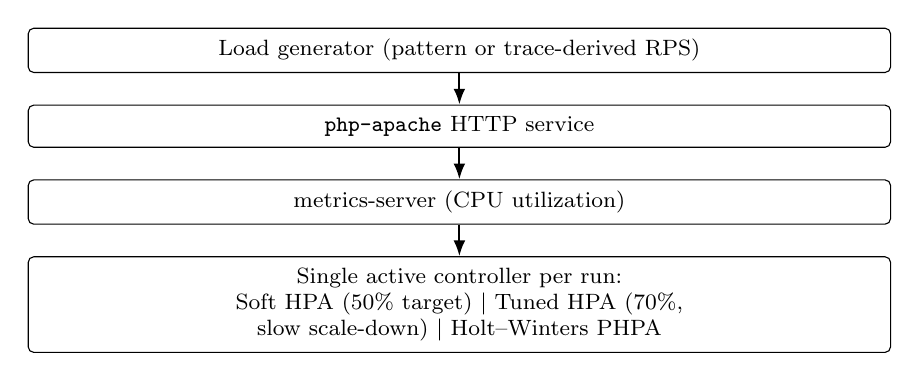
\begin{tikzpicture}[
  font=\footnotesize,
  box/.style={draw, rounded corners=2pt, align=center, inner sep=4pt},
  arr/.style={-{Latex[length=2mm]}, thick},
  node distance=0.4cm
]
\node[box, text width=0.88\columnwidth] (load) {Load generator (pattern or trace-derived RPS)};
\node[box, text width=0.88\columnwidth, below=of load] (app) {\texttt{php-apache} HTTP service};
\node[box, text width=0.88\columnwidth, below=of app] (met) {metrics-server (CPU utilization)};
\node[box, text width=0.88\columnwidth, below=of met] (ctrl) {Single active controller per run:\\
Soft HPA (50\% target) \textbar\ Tuned HPA (70\%, slow scale-down) \textbar\ Holt--Winters PHPA};
\draw[arr] (load) -- (app);
\draw[arr] (app) -- (met);
\draw[arr] (met) -- (ctrl);
\end{tikzpicture}
\caption{Single-controller evaluation on a kind cluster. Load follows either the authors' pattern generator or a frozen trace-derived request schedule.}
\label{fig:arch}
\end{figure}

The tuned HPA configuration is motivated by the observation that the default Kubernetes scale-down stabilization window is 300\,s~\cite{nguyen2020}, and that a 70\% CPU target represents a moderate conservative choice that leaves less idle capacity than 50\% while still providing a margin before saturation~\cite{augustyn2024}. The bounded scale-up (at most four pods per 60\,s) prevents overreaction to single spikes, consistent with recommendations from production Kubernetes operators~\cite{rzadca2020}.

\subsection{Protocol A: historical capacity runs}
For seasonal and burst we use the authors' Makefile-style timings shortened to 120\,s collection, 30\,s warmup, and 5\,s nominal sampling ($n{=}3$ repeats per controller). Metrics are ready pod-seconds (trapezoidal integration on timestamps), hot fraction (share of samples with mean pod CPU above 160\,m), and desired-replica churn. Request latency and errors were \emph{not} recorded in this protocol.

Define Holt--Winters capacity advantage against a reactive arm as $\mathrm{adv}=\mathrm{pod\_s}(\mathrm{reactive})-\mathrm{pod\_s}(\mathrm{HW})$; positive values mean Holt--Winters held less capacity. We report strawman and tuned advantages separately and do \emph{not} use $\mathrm{adv}(\mathrm{strawman})-\mathrm{adv}(\mathrm{tuned})$ because it algebraically equals strawman minus tuned and cancels Holt--Winters.

\subsection{Protocol B: QoS-capable live replays}
A later harness schedules a frozen HTTP request stream, records every request outcome, and integrates ready pod-seconds over a 420\,s measurement window after 120\,s warmup for trace-derived workloads. Error rate uses all scheduled requests; latency percentiles use successful requests only. NASA-derived, Alibaba-derived, on/off, growing, stepped, and guarded chaotic transforms are documented per experiment directory. Original chaotic runs at 20--120\,RPS caused host stress; a separate guarded 10--45\,RPS protocol was used. Rejected, inconclusive, and interrupted runs are excluded from accepted aggregates but retained in the repository.

This two-protocol design reflects the evolution of autoscaling benchmarking methodology: early comparisons focused exclusively on resource utilization~\cite{lorido2014}, while recent work recognizes that capacity alone is insufficient without request-level quality metrics~\cite{mogul2019, mca2026}.

\subsection{Offline forecasting (D1)}
All 600 supplied synthetic scenarios (100 per pattern) are evaluated with rolling-origin forecasts at 15 and 60 minutes (one and four 15-minute steps). Models: persistence, six-sample moving average, fixed-period Holt--Winters, validation-selected Holt--Winters period, and histogram gradient boosting with lag features. Metrics include MAE, RMSE, nonzero-target MAPE, and WAPE. Scenario-level standard deviations describe variation across the 100 scenarios, not repeated execution noise. The Holt--Winters parameters ($\alpha{=}0.9$, $\beta{=}0.2$, $\gamma{=}0.3$) match the PHPA paper's configuration; candidate periods for validation-selected tuning are 6/12/24/48/96.

\subsection{Released online traces (D2)}
We integrate all 42 authors' released CSVs and recompute first-desired-replica-increase timing versus strawman HPA. This verifies released arithmetic; it is not an independent live replication.

\subsection{Real-world forecasting (NASA and Alibaba)}
NASA July 1995 HTTP logs~\cite{arlitt1996} aggregate to complete five-minute request-count bins (7,938 bins; chronological 60/20/20 split). Alibaba uses a bounded v2018 prefix~\cite{jiang2020}: mean \texttt{cpu\_util\_percent} at native ten-second timestamps with at least 20 observed containers per timestamp (3,489 points; same split rule). Horizons are 5 and 60 minutes (NASA) and 10 and 60 seconds (Alibaba). The paper's sub-2\% MAPE claims are \emph{not} reproduced under our targets, splits, and horizons; see the repository's paper-comparison note. Both datasets exhibit the kind of non-stationary behavior that Ali-Eldin et al.~\cite{alieldin2014} characterize as bursty, making them challenging test cases for exponential smoothing methods.

\subsection{Statistics}
Mean $\pm$ sample standard deviation is reported only for genuine repeated groups (historical seasonal/burst, $n{=}3$; NASA soft and Holt--Winters $n{=}3$, tuned $n{=}2$). All other live groups are $n{=}1$ and described without significance testing. Cohen's $d$ is computed for historical pod-second pairs. This conservative statistical reporting follows the recommendation that autoscaling studies should distinguish between descriptive and inferential claims~\cite{mca2026}.

% =============================================================
\section{Results}
% =============================================================

\subsection{Historical seasonal and burst (capacity only)}
Table~\ref{tab:historical} and Fig.~\ref{fig:historical} summarize pod-seconds. On seasonal load, Holt--Winters used 176.21 fewer pod-seconds than strawman HPA on average (Cohen's $d{=}2.44$) but 183.55 \emph{more} than tuned HPA ($d{=}-2.92$). On burst, Holt--Winters beat strawman by 359.86 pod-seconds ($d{=}1.83$) but lost to tuned HPA by 74.98 pod-seconds on average ($d{=}-2.01$); burst repeats overlap and strawman variance is high. Tuned HPA also shows the highest hot fraction, indicating leaner replica counts with busier pods; without request metrics in this protocol we make no SLA claim.

The reversal between strawman and tuned comparisons is the central finding of this protocol: Holt--Winters' capacity advantage is an artifact of the soft 50\% baseline, not an intrinsic property of predictive scaling. This observation directly parallels RLScale-Bench's~\cite{rlscale2026} finding that baseline calibration dominates policy sophistication.

\begin{table}[!t]
\caption{Historical live runs: ready pod-seconds (mean $\pm$ SD, $n{=}3$).}
\label{tab:historical}
\centering
\begin{tabular}{@{}lrrr@{}}
\toprule
Pattern & Soft HPA & Holt--Winters & Tuned HPA \\
\midrule
Seasonal & $943.01 \pm 94.07$ & $766.80 \pm 39.61$ & $583.25 \pm 79.59$ \\
Burst & $1088.25 \pm 274.75$ & $728.38 \pm 46.49$ & $653.40 \pm 24.74$ \\
\bottomrule
\end{tabular}
\end{table}

\begin{figure}[!t]
\centering
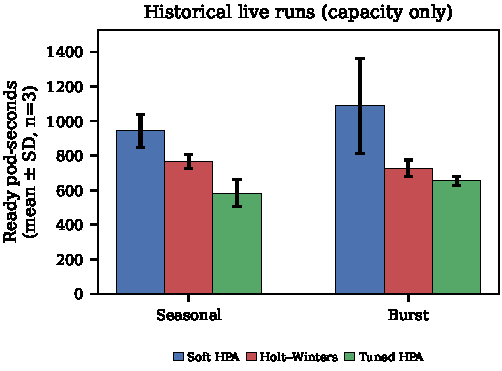
\includegraphics[width=\columnwidth]{figures/fig_historical_pods.pdf}
\caption{Ready pod-seconds on historical seasonal and burst patterns (Protocol~A). Tuned HPA uses fewer pod-seconds than Holt--Winters on both patterns.}
\label{fig:historical}
\end{figure}

\subsection{Offline six-pattern forecasts}
Table~\ref{tab:offline} reports the lowest mean MAE per pattern at the 15-minute horizon. Persistence achieves the best MAE on four of six patterns (burst, chaotic, growing, stepped). GBDT leads on seasonal and on/off. At 60 minutes, burst flips to GBDT leadership (2.30 MAE). These rankings describe forecast error only; they do not establish pod-second or latency superiority of any controller. The dominance of persistence on most patterns at short horizons is consistent with findings from workload characterization studies~\cite{cortez2017, alieldin2014} showing that cloud workloads exhibit high local autocorrelation.

\begin{table}[!t]
\caption{Best model MAE per pattern on D1 synthetic data (15-minute rolling horizon, 100 scenarios each).}
\label{tab:offline}
\centering
\footnotesize
\begin{tabular}{@{}lrr@{}}
\toprule
Pattern & Best model & MAE (mean) \\
\midrule
Burst & Persistence & 1.04 \\
Chaotic & Persistence & 2.67 \\
Growing & Persistence & 0.37 \\
On/off & GBDT & 5.59 \\
Seasonal & GBDT & 0.53 \\
Stepped & Persistence & 0.61 \\
\bottomrule
\end{tabular}
\end{table}

\begin{figure}[!t]
\centering
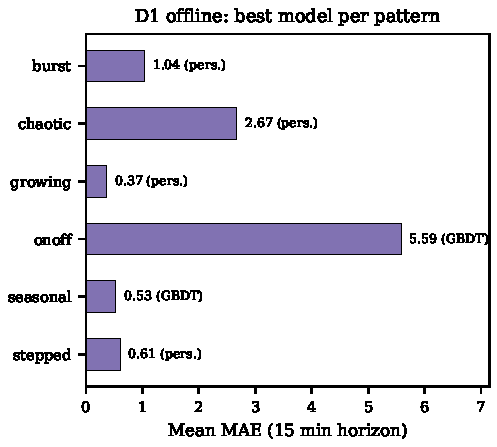
\includegraphics[width=\columnwidth]{figures/fig_offline_mae.pdf}
\caption{Lowest mean MAE per pattern on D1 synthetic data (15-minute horizon). Parentheses name the winning model variant.}
\label{fig:offline}
\end{figure}

\subsection{Released early-detection audit}
Recomputed first-desired-increase advantages for Holt--Winters versus strawman HPA on authors' released traces: burst 20.48\,s; chaotic 30.85\,s; growing 30.72\,s; on/off 40.93\,s; seasonal 30.77\,s; stepped 30.71\,s (matches rounded paper/Kaggle values within 0.05\,s). These timing advantages must be interpreted with caution: earlier scaling may reflect higher starting replicas, controller cadence, or more aggressive scaling parameters rather than genuine workload anticipation. We did not remeasure early detection in our shortened 120\,s historical windows.

\subsection{QoS-capable live replays}
Table~\ref{tab:live} lists accepted overload-oriented outcomes. These results reveal a consistent capacity--QoS tradeoff conditioned on workload stress level.

\textbf{NASA-derived overload.} Holt--Winters reduced error rate to $18.04\% \pm 2.05\%$ versus $44.76\% \pm 9.37\%$ for soft HPA and $37.75\% \pm 2.34\%$ for tuned HPA ($n{=}3$, $n{=}2$, $n{=}3$ respectively), with successful-request p95 latency $0.868 \pm 0.653$\,s versus $2.508 \pm 0.918$\,s and $2.241 \pm 0.306$\,s, at roughly $3.5\times$ the pod-seconds of soft HPA. This demonstrates that predictive scaling can materially reduce request errors under sustained overload, consistent with the proactive provisioning advantage described by Abdullah et al.~\cite{abdullah2022}.

\textbf{On/off and stepped.} On/off shows a similar capacity--QoS tradeoff: Holt--Winters errors $13.29\%$ versus tuned $48.55\%$ but $165.9\%$ more pod-seconds than tuned ($n{=}1$). On stepped plateaus, accepted tuned HPA had $17.58\%$ errors versus $1.01\%$ for Holt--Winters at $+121.8\%$ pod-seconds; soft HPA was \emph{rejected} because generator dispatch p99 exceeded the frozen integrity threshold (its descriptive error rate is not promoted to the accepted matrix).

\textbf{Zero-error workloads.} Growing and Alibaba-derived replays recorded zero request errors for all accepted arms; tuned HPA used the fewest pod-seconds on growing ($1572.5$ vs.\ $1927.5$ soft and $2897.5$ Holt--Winters). Guarded chaotic (10--45\,RPS) succeeded for all three controllers with tuned HPA leanest on pod-seconds ($990.0$ vs.\ $1185.0$ soft and $1342.5$ Holt--Winters). Original 20--120\,RPS chaotic soft HPA showed $85.47\%$ errors; Holt--Winters attempts froze the host and tuned HPA was not run---no cross-controller conclusion is drawn for that protocol. These zero-error results are particularly important: when the workload is serviceable without predictive overprovisioning, the predictor's extra capacity provides no observable QoS benefit.

\begin{table}[!t]
\caption{Selected QoS-capable live replays (Protocol~B). NASA rows: mean $\pm$ SD.}
\label{tab:live}
\centering
\footnotesize
\setlength{\tabcolsep}{3pt}
\adjustbox{width=\columnwidth,center}{%
\begin{tabular}{@{}p{0.19\columnwidth}p{0.22\columnwidth}rrr@{}}
\toprule
Workload & Controller & Err.\ (\%) & p95 (s) & Pod-s \\
\midrule
NASA & Soft HPA & 44.8$\pm$9.4 & 2.51$\pm$0.92 & 1193$\pm$156 \\
NASA & Tuned HPA & 37.8$\pm$2.3 & 2.24$\pm$0.31 & 915$\pm$18 \\
NASA & Holt--Winters & 18.0$\pm$2.1 & 0.87$\pm$0.65 & 3479$\pm$20 \\
On/off & Holt--Winters & 13.29 & 0.050 & 3542.5 \\
On/off & Tuned HPA & 48.55 & 1.069 & 1332.5 \\
Stepped & Tuned HPA & 17.58 & 0.011 & 5872.5 \\
Stepped & Holt--Winters & 1.01 & 0.016 & 13025.0 \\
\bottomrule
\end{tabular}%
}
\end{table}

\begin{figure}[!t]
\centering
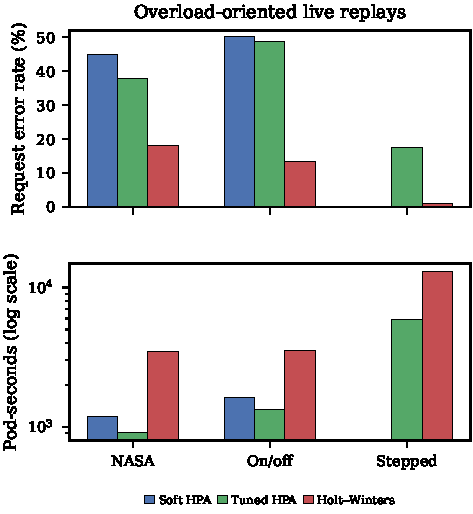
\includegraphics[width=\columnwidth]{figures/fig_live_qos.pdf}
\caption{Request error rate (top) and pod-seconds on a log scale (bottom) for overload-oriented replays. Stepped soft HPA omitted (rejected run).}
\label{fig:liveqos}
\end{figure}

\subsection{Real-world held-out forecasting}
Table~\ref{tab:rw} reports best gradient-boosted tree MAE on held-out test folds. NASA request counts and Alibaba CPU percentages are not pooled. Exponential smoothing nearly matches GBDT (within a few percent MAE); our MAPE values remain far from the paper's sub-2\% headline because targets, splits, horizons, and features differ. The relatively small gap between simple exponential smoothing and GBDT on these real-world datasets parallels Imdoukh et al.'s~\cite{imdoukh2020} observation that model complexity does not always translate to proportionate accuracy gains for cloud workload prediction.

\begin{table}[!t]
\caption{Held-out forecasting (GBDT best MAE; WAPE in percent).}
\label{tab:rw}
\centering
\footnotesize
\adjustbox{width=\columnwidth,center}{%
\begin{tabular}{@{}p{0.28\columnwidth}p{0.14\columnwidth}rrr@{}}
\toprule
Dataset & Horizon & MAE & RMSE & WAPE \\
\midrule
NASA (req./5\,min) & 5\,min & 36.32 & 47.82 & 18.51 \\
NASA (req./5\,min) & 60\,min & 50.83 & 66.61 & 25.85 \\
Alibaba (CPU \%) & 10\,s & 1.72 & 2.13 & 14.49 \\
Alibaba (CPU \%) & 60\,s & 1.73 & 2.13 & 14.52 \\
\bottomrule
\end{tabular}%
}
\end{table}

\subsection{Ablation (derived arms)}
Component~B uses Holt--Winters on seasonal and strawman HPA on burst (pod-seconds $766.80 \pm 39.61$ and $1088.25 \pm 274.75$). Components~A+B use Holt--Winters on seasonal and tuned HPA on burst ($766.80 \pm 39.61$ and $653.40 \pm 24.74$). These reuse measured runs; they do not add new cluster experiments. The pattern-switch ablation demonstrates that oracle pattern knowledge combined with calibrated reactive control (Components~A+B) achieves the best capacity across both patterns---Holt--Winters' seasonal advantage is preserved while burst capacity waste is eliminated by using the tuned reactive controller.

Table~\ref{tab:ablation} summarizes the four system configurations and their total pod-seconds across both patterns.

\begin{table}[!t]
\caption{Ablation: total pod-seconds across seasonal and burst (derived from measured runs).}
\label{tab:ablation}
\centering
\footnotesize
\begin{tabular}{@{}llrr@{}}
\toprule
System & seasonal & burst & total \\
\midrule
Strawman vs HW & 943.01 & 1088.25 & 2031.26 \\
Orig.\ + Comp.~A & 583.25 & 653.40 & 1236.65 \\
Orig.\ + Comp.~B & 766.80 & 1088.25 & 1855.05 \\
Orig.\ + A + B & 766.80 & 653.40 & 1420.20 \\
\bottomrule
\end{tabular}
\end{table}

% =============================================================
\section{Discussion}
% =============================================================

\subsection{Calibration matters}
Against the authors' 50\% HPA, Holt--Winters often looks favorable on pod-seconds (historical seasonal/burst). Against our single conservative tune, that capacity advantage reverses on both historical patterns. This supports RLScale-Bench's~\cite{rlscale2026} warning that reactive baseline choice dominates naive predictive comparisons. The finding also aligns with the broader observation from Qu et al.~\cite{qu2018} that autoscaling benchmarks are highly sensitive to experimental setup choices, and with Bauer et al.'s~\cite{bauer2017} recommendation for application-aware baselines.

Our tuned HPA uses a 70\% CPU target---higher than the 50\% strawman but still conservative relative to production practice. The 300\,s scale-down stabilization matches the Kubernetes default, yet this single documented change suffices to reverse the capacity comparison. Practitioners should note that the calibration effort is minimal: a single configuration change, not a model training pipeline.

\subsection{QoS appears only under stress}
When all controllers already serve every request (growing, Alibaba-derived, guarded chaotic), predictive scaling does not improve observed errors but still costs capacity in several cases. Under NASA-derived and on/off overload, Holt--Winters materially reduces errors and latency at a large pod-second cost---a capacity--QoS tradeoff, not universal predictive dominance. This conditional advantage is consistent with the proactive scaling literature~\cite{abdullah2022, pahpa2026}: the value of prediction depends on whether the system would otherwise be overloaded.

The workload-dependent nature of the advantage has practical implications. Organizations operating services with known overload risk (e.g., flash sales, viral content) may benefit from predictive scaling despite its cost. Services with stable or gradually evolving demand may find a tuned reactive baseline sufficient, avoiding the operational complexity of maintaining a prediction model~\cite{rzadca2020}.

\subsection{Forecast accuracy does not equal policy quality}
Offline persistence wins on four patterns at 15 minutes; GBDT wins seasonal and on/off. None of these tables substitute for live autoscaling outcomes. The gap between forecast accuracy and autoscaling quality has been noted in several contexts~\cite{cortez2017, mca2026}: a more accurate forecast does not guarantee better scaling if the controller policy, stabilization parameters, or scaling granularity mask the forecast improvement. Our results provide concrete evidence for this gap across six workload patterns.

\subsection{Anticipation versus aggressiveness}
Earlier replica changes on released traces and in some live runs may reflect higher starting replicas, controller cadence, or aggressive scaling rather than correct peak prediction; stepped upward transitions showed no desired-replica increases in the 60\,s before the analyzed step for accepted arms. This distinction between genuine anticipation and incidental early scaling is critical for interpreting the PHPA paper's early-detection metric: a controller that always maintains high replica counts will trivially ``detect'' load increases early, but this is overprovisioning rather than prediction.

\subsection{Pattern-dependent recommendations}
Based on our evidence, we offer the following tentative pattern-level guidance for practitioners choosing between reactive and predictive HPA:
\begin{itemize}
\item \textbf{Seasonal/burst (low stress):} Tuned reactive HPA is sufficient. Predictive scaling adds cost without measurable QoS benefit.
\item \textbf{On/off and stepped (overload risk):} Holt--Winters materially reduces errors. The capacity cost may be justified by SLA requirements.
\item \textbf{Growing:} Gradual demand increase is well-handled by reactive scaling. Predictive scaling adds unnecessary capacity.
\item \textbf{Chaotic:} Insufficient evidence; host-level instability prevented complete evaluation.
\end{itemize}
These recommendations are bounded to our experimental conditions and should be validated in production environments with production-grade cluster configurations.

% =============================================================
\section{Limitations}
% =============================================================
Several limitations constrain the generalizability of our findings.

\textbf{Experimental scope.} Shortened 120\,s historical windows versus the authors' 300\,s; Holt--Winters seasonal period six (60\,s) versus $\approx$80\,s seasonal generator period; single-node kind on laptops; fixed run order; $n{=}1$ for most QoS replays; inconclusive NASA tuned third repeat; chaotic host freezes; no LLM path; one tuned HPA configuration rather than a sweep; affine trace-to-RPS mappings that are not production workloads.

\textbf{Baseline selection.} We evaluate a single tuned HPA configuration. A systematic sweep over CPU targets, stabilization windows, and scaling rates---as recommended by Augustyn et al.~\cite{augustyn2024}---might identify configurations that further narrow or widen the gap with Holt--Winters. Our finding that \emph{one} documented tune reverses the capacity comparison is a lower bound on what calibration can achieve.

\textbf{Predictor configuration.} The Holt--Winters parameters are fixed from the original paper and are not retuned for our cluster or workloads. A per-pattern or per-workload parameter search might improve predictive performance, though this would also increase operational complexity.

\textbf{Workload realism.} Our replays use synthetic and trace-derived request schedules with affine RPS mappings, not genuine production traffic. The growing, on/off, stepped, and chaotic patterns are idealized mathematical functions. Real-world workloads exhibit more complex dynamics~\cite{cortez2017, jiang2020} that may favor or disfavor predictive approaches differently.

\textbf{Cluster environment.} A single-node kind cluster cannot reproduce the scheduling, networking, and resource contention characteristics of multi-node production Kubernetes clusters. Pod startup times, CPU throttling, and metrics-server latency may all differ in production~\cite{dogani2023}.

\textbf{Missing metrics.} Historical runs lack request-level QoS. The hot-fraction metric indicates per-pod load intensity but does not substitute for measured service quality. Per-request backend identity is not available, preventing attribution of errors to specific pod states.

% =============================================================
\section{Conclusion}
% =============================================================
We provide a reproducible, pattern-stratified benchmark that reproduces PHPA's Holt--Winters versus strawman HPA comparison and asks whether a conservatively tuned HPA changes the conclusion. Measured evidence shows tuned reactive control is more capacity-efficient than Holt--Winters on the historical seasonal and burst patterns and on several successful low-error replays, while Holt--Winters improves errors and latency under sustained overload at substantially higher pod-seconds.

The key insight is workload-conditional: predictive autoscaling's value depends on whether the system faces genuine overload that reactive scaling cannot resolve. When a tuned reactive controller already serves the workload successfully, prediction adds cost without measurable benefit. This finding extends the calibrated-baseline critique from RL-based autoscaling~\cite{rlscale2026} to lightweight time-series predictors, and supports the growing consensus~\cite{mca2026, qu2018, dogani2023} that autoscaling research must evaluate against honestly configured baselines across diverse workload regimes.

Practitioners should treat predictive autoscaling as a workload- and calibration-dependent capacity--QoS tradeoff rather than a default upgrade over tuned reactive HPA. Future work should evaluate additional predictive models (LSTM, Transformer-based), perform systematic HPA parameter sweeps, and test on multi-node clusters with production traffic to establish more general guidelines.

\section*{Reproducibility}
The public repository documents environment setup, verification commands, per-experiment \texttt{REPRODUCE.md} files, and the \texttt{plot\_paper\_figures.py} script used to regenerate bar charts. Accepted measurement CSVs are retained rather than overwritten. All code and instructions are available at \url{https://github.com/umaritics/calibrated-autoscaling-benchmark}.

% =============================================================
% REFERENCES
% =============================================================
\begin{thebibliography}{99}

\bibitem{duman2026}
C.~Duman and S.~Eken, ``From Reactive to Predictive: A Pattern-Aware Framework for Kubernetes Autoscaling with Large Language Model Integration,'' \emph{J. Syst. Softw.}, vol.~237, 2026, doi:10.1016/j.jss.2026.112861.

\bibitem{rlscale2026}
G.~Zhang, C.~Sun, K.~Zhao, X.~Chu, S.~Sarkani, and J.~M.~Fossaceca, ``When Does Deep RL Beat Calibrated Baselines? A Benchmark Study on Adaptive Resource Control,'' arXiv preprint arXiv:2605.26418, 2026, doi:10.48550/arXiv.2605.26418.

\bibitem{adapt2026}
H.~S.~Baghel, ``ADAPT: A Self-Calibrating Proactive Autoscaler for Container Orchestration,'' arXiv preprint arXiv:2605.15788, 2026, doi:10.48550/arXiv.2605.15788.

\bibitem{arascaler2025}
B.~Jeong and Y.-S.~Jeong, ``ARAScaler: Adaptive Resource Autoscaling Scheme Using ETimeMixer for Efficient Cloud-Native Computing,'' \emph{IEEE Trans. Services Comput.}, vol.~18, no.~1, pp.~72--84, 2025, doi:10.1109/TSC.2024.3522815.

\bibitem{mca2026}
V.~S.~Machiraju, V.~Kumar, and S.~Sharma, ``ML-Based Autoscaling for Elastic Cloud Applications: Taxonomy, Frameworks, and Evaluation,'' \emph{Math. Comput. Appl.}, vol.~31, no.~2, art.~49, 2026, doi:10.3390/mca31020049.

\bibitem{kumar2026}
B.~Kumar, A.~Verma, and R.~Buyya, ``Predictive Autoscaling in Cloud-Native and Federated Cloud-Edge Computing Environments: A Taxonomy and Future Directions,'' arXiv preprint arXiv:2606.07046, 2026, doi:10.48550/arXiv.2606.07046.

\bibitem{schroder2023}
C.~Schr\"oder, R.~B\"ohm, and A.~Lampe, ``Comparison of Autoscaling Frameworks for Containerised Machine-Learning Applications in a Local and Cloud Environment,'' arXiv preprint arXiv:2311.18659, 2023, doi:10.48550/arXiv.2311.18659.

\bibitem{lorido2014}
T.~Lorido-Botran, J.~Miguel-Alonso, and J.~A.~Lozano, ``A Review of Auto-scaling Techniques for Elastic Applications in Cloud Environments,'' \emph{J. Grid Comput.}, vol.~12, no.~4, pp.~559--592, 2014, doi:10.1007/s10723-014-9314-7.

\bibitem{qu2018}
C.~Qu, R.~N.~Calheiros, and R.~Buyya, ``Auto-Scaling Web Applications in Clouds: A Taxonomy and Survey,'' \emph{ACM Comput. Surv.}, vol.~51, no.~4, art.~73, pp.~1--33, 2018, doi:10.1145/3148149.

\bibitem{rzadca2020}
K.~Rz\k{a}dca, P.~Findeisen, J.~\'Swiderski, P.~Zych, P.~Broniek, J.~Ku\'smierek, P.~K.~Nowak, B.~Strack, P.~Witusowski, S.~Hand, and J.~Wilkes, ``Autopilot: Workload Autoscaling at Google,'' in \emph{Proc. EuroSys}, 2020, doi:10.1145/3342195.3387524.

\bibitem{mogul2019}
J.~C.~Mogul and J.~Wilkes, ``Nines are Not Enough: Meaningful Metrics for Clouds,'' in \emph{Proc. HotOS}, pp.~136--141, 2019, doi:10.1145/3317550.3321432.

\bibitem{herbst2013}
N.~R.~Herbst, S.~Kounev, and R.~Reussner, ``Elasticity in Cloud Computing: What It Is, and What It Is Not,'' in \emph{Proc. ICAC}, pp.~23--27, 2013, doi:10.5555/2500798.00005.

\bibitem{augustyn2024}
D.~R.~Augustyn, \L.~Wyci\'slik, and M.~Sojka, ``Tuning a Kubernetes Horizontal Pod Autoscaler for Meeting Performance and Load Demands in Cloud Deployments,'' \emph{Appl. Sci.}, vol.~14, no.~2, art.~646, 2024, doi:10.3390/app14020646.

\bibitem{shahin2016}
A.~A.~Shahin, ``Using Multiple Seasonal Holt-Winters Exponential Smoothing to Predict Cloud Resource Provisioning,'' \emph{Int. J. Adv. Comput. Sci. Appl.}, vol.~7, no.~11, 2016, doi:10.14569/IJACSA.2016.071113.

\bibitem{imdoukh2020}
M.~Imdoukh, I.~Ahmad, and M.~Gh.~Alfailakawi, ``Machine Learning-Based Auto-Scaling for Containerized Applications,'' \emph{Neural Comput. Appl.}, vol.~32, pp.~9745--9760, 2020, doi:10.1007/s00521-019-04513-x.

\bibitem{mondal2023}
S.~K.~Mondal \emph{et al.}, ``Toward Optimal Load Prediction and Customizable Autoscaling Scheme for Kubernetes,'' \emph{Mathematics}, vol.~11, no.~12, art.~2675, 2023, doi:10.3390/math11122675.

\bibitem{rubak2023}
A.~Rubak and J.~Taheri, ``Machine Learning for Predictive Resource Scaling of Microservices on Kubernetes Platforms,'' in \emph{Proc. IEEE/ACM UCC}, 2023, doi:10.1145/3603166.3632165.

\bibitem{pahpa2026}
J.~Xiao, F.~Yang, W.~Ai, T.~Meng, and G.~Xie, ``PAHPA: Revolutionizing Kubernetes Autoscaling With Integrated Predictive Analytics and Real-Time Monitoring,'' \emph{IEEE Trans. Services Comput.}, vol.~19, no.~3, pp.~2343--2355, 2026, doi:10.1109/TSC.2026.3685325.

\bibitem{bacc2026}
F.~Liu, G.~Li, B.~Farkiani, and P.~Crowley, ``BACC: Budget-Aware Calibration and Control for Horizontal Autoscaling,'' arXiv preprint arXiv:2606.20575, 2026, doi:10.48550/arXiv.2606.20575.

\bibitem{abdullah2022}
M.~Abdullah, W.~Iqbal, J.~L.~Berral, J.~Polo, and D.~Carrera, ``Burst-Aware Predictive Autoscaling for Containerized Microservices,'' \emph{IEEE Trans. Services Comput.}, vol.~15, no.~3, pp.~1448--1460, 2022, doi:10.1109/TSC.2020.2995937.

\bibitem{base2026}
C.~Meng, H.~Tong, T.~Wu, M.~Pan, Y.~Yu, and Y.~Jiang, ``BASE: Burst-Adaptive Autoscaling via Stacked Ensembles for SLO Assurance and Cost Efficiency,'' \emph{IEEE Trans. Services Comput.}, vol.~19, no.~2, pp.~963--976, 2026, doi:10.1109/TSC.2026.3668105.

\bibitem{santos2023}
J.~Santos, T.~Wauters, B.~Volckaert, and F.~De~Turck, ``gym-hpa: Efficient Auto-Scaling via Reinforcement Learning for Complex Microservice-based Applications in Kubernetes,'' in \emph{Proc. IEEE/IFIP NOMS}, 2023, doi:10.1109/NOMS56928.2023.10154298.

\bibitem{rossi2023}
F.~Rossi, V.~Cardellini, F.~Lo~Presti, and M.~Nardelli, ``Dynamic Multi-Metric Thresholds for Scaling Applications Using Reinforcement Learning,'' \emph{IEEE Trans. Cloud Comput.}, vol.~11, no.~2, pp.~1807--1821, 2023, doi:10.1109/TCC.2022.3163357.

\bibitem{park2024}
J.~Park, B.~Choi, C.~Lee, and D.~Han, ``Graph Neural Network-Based SLO-Aware Proactive Resource Autoscaling Framework for Microservices,'' \emph{IEEE/ACM Trans. Netw.}, vol.~32, no.~4, pp.~3331--3346, 2024, doi:10.1109/TNET.2024.3393427.

\bibitem{wang2024}
Z.~Wang \emph{et al.}, ``DeepScaling: Autoscaling Microservices With Stable CPU Utilization for Large Scale Production Cloud Systems,'' \emph{IEEE/ACM Trans. Netw.}, vol.~32, no.~5, pp.~3961--3976, 2024, doi:10.1109/TNET.2024.3400953.

\bibitem{arlitt1996}
M.~F.~Arlitt and C.~L.~Williamson, ``Web Server Workload Characterization: The Search for Invariants,'' in \emph{Proc. ACM SIGMETRICS}, pp.~126--137, 1996, doi:10.1145/233013.233034.

\bibitem{jiang2020}
C.~Jiang, Y.~Qiu, W.~Shi, \emph{et al.}, ``Characterizing Co-Located Workloads in Alibaba Cloud Datacenters,'' \emph{IEEE Trans. Cloud Comput.}, 2020, doi:10.1109/TCC.2020.3034500.

\bibitem{cortez2017}
E.~Cortez, A.~Bonde, A.~Muzio, M.~Russinovich, M.~Fontoura, and R.~Bianchini, ``Resource Central: Understanding and Predicting Workloads for Improved Resource Management in Large Cloud Platforms,'' in \emph{Proc. ACM SOSP}, 2017, doi:10.1145/3132747.3132772.

\bibitem{alieldin2014}
A.~Ali-Eldin, O.~Seleznjev, S.~Sj\"ostedt-de~Luna, J.~Tordsson, and E.~Elmroth, ``Measuring Cloud Workload Burstiness,'' in \emph{Proc. IEEE/ACM UCC}, pp.~566--572, 2014, doi:10.1109/UCC.2014.87.

\bibitem{dogani2023}
J.~Dogani, R.~Namvar, and F.~Khunjush, ``Auto-Scaling Techniques in Container-Based Cloud and Edge/Fog Computing: Taxonomy and Survey,'' \emph{Comput. Commun.}, vol.~209, pp.~120--150, 2023, doi:10.1016/j.comcom.2023.06.010.

\bibitem{bauer2017}
A.~Bauer, N.~Herbst, and S.~Kounev, ``Design and Evaluation of a Proactive, Application-Aware Auto-Scaler,'' in \emph{Proc. ICPE}, 2017, doi:10.1145/3030207.3053678.

\bibitem{nguyen2020}
T.-T.~Nguyen, Y.-J.~Yeom, T.~Kim, D.-H.~Park, and S.~Kim, ``Horizontal Pod Autoscaling in Kubernetes for Elastic Container Orchestration,'' \emph{Sensors}, vol.~20, no.~16, art.~4621, 2020, doi:10.3390/s20164621.

\bibitem{carrion2022}
C.~Carri\'on, ``Kubernetes Scheduling: Taxonomy, Ongoing Issues and Challenges,'' \emph{ACM Comput. Surv.}, vol.~55, no.~7, art.~146, pp.~1--37, 2022, doi:10.1145/3539606.

\end{thebibliography}

\end{document}
